\documentclass[9pt,conference]{IEEEtran}
\usepackage[utf8]{inputenc}
\usepackage[brazil]{babel}

% Diversos
\usepackage{csquotes}
\usepackage{graphicx}
\usepackage{verbatim}
\usepackage{hyperref}
\usepackage{smartdiagram}

% Título
\title{Utilizando Redes Convolucionais de Grafos Espaço-Temporais para o Reconhecimento da Línguas de Sinais}
%\author{Cleison Correia de Amorim}
\date{Outubro 2018}

\author{
    \IEEEauthorblockN{Cleison Correia de Amorim}
    \IEEEauthorblockA{Centro de Informática\\
    Universidade Federal de Pernambuco\\
    Email: cca5@cin.ufpe.br}
}

% Comandos
% 'image': definição de imagem
\newcommand{\image}[4][\linewidth] {
    \begin{figure}[ht]
    \centering
    \includegraphics[width=#1]{#3}
    \caption{#4}
    \label{#2}
    \end{figure}
}

% 'refimage': referências de imagens
\newcommand{\refimage}[1] {figura \ref{#1}}

% 'refsection': referências de seções
\newcommand{\refsect}[1] {seção "\nameref{#1}"}


\begin{document}
\maketitle

%%%%%%%%%%%%%%%%%%%%%%%%%%%%%%%%%%%%%%%%%%%%%%%%%%%%%%%%%%%%%%%%%%%%%%%%%
% Abstract:
\begin{abstract}
The recognition of sign language is a field of research with several challenges, but it has an important role to facilitate the communication of the Deaf and to remove the barriers in this communication to society. This paper presents the application of a deep learning algorithm known as Spatial Temporal Graph Convolutional Network to promote the recognition of this language. This is a new approach centered on human skeletal movement that uses graphs to capture its dynamics in two dimensions, spatial and temporal, and that is able to consider complex aspects of the context of signs. Additionally, this paper presents the creation of a dataset of human skeletons for sign language that is based on ASLLVD, and which, in addition to being used in this study, is publicly available to contribute to future related studies.
\end{abstract}

%%%%%%%%%%%%%%%%%%%%%%%%%%%%%%%%%%%%%%%%%%%%%%%%%%%%%%%%%%%%%%%%%%%%%%%%%
% Keywords:
\begin{IEEEkeywords}
Sign Language, Convolutional Neural Network, Spatial Temporal Graph.
\end{IEEEkeywords}


%%%%%%%%%%%%%%%%%%%%%%%%%%%%%%%%%%%%%%%%%%%%%%%%%%%%%%%%%%%%%%%%%%%%%%%%%
\section{Introduction} 
\label{sec:introducao}

Sign language is a visual communication tool that enables individuals with different types of hearing impairment to communicate with other individuals in society. It is the language used by most Deaf people in their daily lives and, moreover, it is the symbol of identification between the members of that community and the main force that unites them.  It has a very close relationship with the culture of the countries where it is used and for this reason each of these nations has its own language born and developed with its Deaf communities \cite{pereira-choi-2011}.

According to the World Health Organization, the number of deaf people is about 466 million and it estimates that by 2050 this number exceeds 900 million -- which is equivalent to a forecast of 1 in 10 individuals around the world \cite{who-2018}. These data, in turn, highlight the breadth and importance of the sign language in the communication of these people in different nations.

Despite this, there is still a small number of hearing people who are able to communicate through that language. This ends up characterizing an invisible barrier that interferes with the communication between deaf and hearing, making a more effective integration between these people impossible \cite{peres-2006}. In this context, it is extremely important to develop tools that are able to fill this gap by promoting integration among these people.

For this reason, studies related to the recognition of signs have been developed since the 1990s and it is possible to verify significant results from them \cite{lim-2016, recent-advances-dl-2017}. The main challenges encountered are primarily related to the need to consider the dynamic aspects of the language, such as movements, articulations between body parts and non-manual expressions, rather than simply recognizing static signs or isolated hand positions. In addition, that language has thousands of signs, which sometimes differ only by subtle changes in movement, shape, or position of the hands and involve significant overlaps of fingers and occlusions. When combined with differences in signing style by distinct individuals and the variations arising from its non-universality and regionalisms, this field of research can become really challenging for current artificial intelligence algorithms \cite{konstantinidis-2018}.

This work, therefore, presents the application in this area of research of a new approach capable of performing the recognition of human actions based on spatial-temporal graphs, which is called Spatial-Temporal Graph Convolutional Networks (ST-GCN) \cite {st-gcn-2018}. Using graph representations of human skeleton, this technique focuses on body movement and the interactions between its parts, disregarding the interference of the environment around them. In addition, it also addresses the movements under the spatial and temporal dimensions, and this allows them to capture the dynamic aspects of the actions exercised over time. These characteristics make this a very relevant approach to dealing with the challenges and peculiarities of sign language recognition.

In order to apply the above method, however, it was first necessary to develop a dataset of human skeletons for the sign language that would serve as the main information to feed the ST-GCN and enable the creation of its graphs. For this, the American Sign Language Lexicon Video Dataset (ASLLVD) was used. It consists of a large set of signs of the American Sign Language (ASL), from which the necessary skeletons were segmented and estimated.

Thus, this work has as main contributions: 1) the adoption in the domain of sign recognition of a new technique centered on human movement, which considers different aspects of its dynamics and contributes to overcome some of the main challenges mentioned above; 2) the creation of a new dataset of human skeletons for sign language, currently non-existent, which aims to support the development of studies in this area.

This work is organized as follows: section  \ref{sec:trabalhos-relacionados} presents the related works and details of the operation of the ST-GCN; section \ref{sec:experimentos} addresses the conduction of the experiments, including the creation of the new dataset and the adjustments made in ST-GCN; Finally, section \ref{sec:resultados} contains the results obtained from the applied approach.


%%%%%%%%%%%%%%%%%%%%%%%%%%%%%%%%%%%%%%%%%%%%%%%%%%%%%%%%%%%%%%%%%%%%%%%%%
\section{Related work}
\label{sec:trabalhos-relacionados}

The recognition of sign languages has made significant progress in recent years, which are motivated mainly by the advent of modern sensors, new machine learning techniques and more powerful hardware that allow the emergence of more robust algorithms \cite{recent-advances-dl-2017, recent-advances-sl-2013}. In addition, approaches considered intrusive and requiring the use of sensors such as gloves, accelerometers and markers coupled to the body of the interlocutor have been gradually abandoned, giving way to new approaches using conventional cameras and computer vision techniques.

Due to this movement, it is also noticeable the increase in the adoption of techniques for feature extraction such as SIFT \cite{lowe-2004}, HOG \cite{dalal-2005}, HOF \cite{laptev-2008} and STIP \cite{laptev-2008} in order to preprocess the images obtained by these cameras and provide richer information for use by the learning algorithms \cite{lim-2016, shanta-2018}.

Convolutional Neural Networks (CNNs), in turn, have recently stood out as the algorithm with more expressive presence in this field. Its results have been remarkable and its accuracy is generally reaches 90\% \cite{shanta-2018, ji-2017, taskiran-2018, rao-2018}. Some of its variations also found are the 3D CNNs \cite{elbadawy-2017}, the combination with other models like Inception \cite{das-2018} or the Regions of Interest application \cite{sajanraj-2018}. To a lesser extent, it is also noted the adoption of Recurrent Neural Networks \cite{konstantinidis-2018} and Temporal Residual Networks \cite{pigou-2017} for the same purpose.

Despite the above advances, a large portion of these studies is still restricted to addressing this problem by means of static or single-letter images, from the datylology\footnote{
     Datylology - also known as digital or manual alphabet. It consists in the spelling of words by the Deaf. It is generally used to introduce a word that does not yet have an equivalent sign \cite{quadros-2004, pereira-choi-2011}.
} \cite{shanta-2018, taskiran-2018, elbadawy-2017, das-2018, sajanraj-2018}. This is negative because it causes the intrinsic dynamics of the language, such as its movements, non-manual expressions and articulations between parts of the body, to be disregarded \cite{quadros-2004}. In this sense, it is extremely relevant that new studies are able to observe such important characteristics, as in \cite{konstantinidis-2018} and \cite {pigou-2017}.

With this purpose, the current work presents the use of an approach centered on body skeletal movement to perform sign recognition. This technique is known as Spatial-Temporal Graph Convolutional Network (ST-GCN)\footnote {
    Available at \url{https://github.com/yysijie/st-gcn}.
} and was introduced in \cite{st-gcn-2018}. Its motivation, according to its authors, arose from the need for methods that were capable of autonomously capturing the patterns contained in the spatial configuration of the body joints as well as their temporal dynamics. They argue that previous methods for action recognition were limited by not explicitly exploring such spatial relations between the joints, which are crucial for the understanding of human actions. These methods simply used the joint coordinates in individual time steps to form feature vectors, applying a temporal analysis on them \cite{st-gcn-2018, wang-2012, fernando-2015}.

The ST-GCN uses as base of its formulation a sequence of skeleton graphs representing the human body, which is obtained from a series of action frames of individuals. Figure \ref{fig:st-gcn-graph} allows us to visualize this structure, where each node corresponds to a point of articulation. The intra-body vertices are defined based on the body's natural connections. The inter-frame vertices, in turn, connect the same joints between consecutive frames to denote their trajectory over time \cite{st-gcn-2018}.

\image
	[3.5cm]
    {fig:st-gcn-graph}
    {images/st_gcn_graph}
    {Sequence of skeleton graphs, denoting human movement in space and time, used by the ST-GCN \cite[p. 1]{st-gcn-2018}.}

Figure \ref{fig:st-gcn-workflow} gives an overview of the approach used by this technique. First, the estimation of individuals' skeletons in the input videos is carried out, as well as the construction of space-time graphs based on them. Then, multiple ST-GCN convolution layers are applied, gradually generating higher and higher level feature maps for the presented graphs. Finally, they are submitted to a classifier to identify the corresponding action.

\image
    {fig:st-gcn-workflow}
    {images/st_gcn_workflow}
    {Graphs created from skeletons of individuals in the videos are submitted to consecutive layers of ST-GCN convolution and, finally, classified among the available actions \cite[p. 3]{st-gcn-2018}.}

To understand the operation of the ST-GCN, it is necessary first to introduce its sampling and partitioning strategies. When we are dealing with convolutions over 2D images, it is easy to imagine the existence of a rigid grid (or rectangle) around a central point that represents the sampling area of the convolutional filter, which delimits its neighborhood. In the case of graphs, however, it is necessary to go beyond this definition and to consider that the neighborhood of the center point will now be composed of points that are directly connected by a vertex. Figure \ref{fig:st-gcn-sampling} allows us to visualize this definition for a single frame. Note that for the red center points, the dashed edges will then represent the sampling area of the convolutional filter. Note also that although there are other points physically close to the central points (such as the points of the feet, knees and waist), they will not be considered unless there is a vertex connecting them to the points in red. This is the \textbf{sampling strategy} adopted by ST-GCN.

\image
	[2.5cm]
    {fig:st-gcn-sampling}
    {images/st_gcn_sampling}
    {Sampling strategy in a convolution for a single frame. The body joints are drawn with blue dots. The red dots represent the center points of a filter with distance D = 1 applied to the graph, whose range is delimited by the dashed line \cite[p. 5]{st-gcn-2018}.}

From figure \ref{fig:st-gcn-sampling} it is possible to observe that only points immediately connected to the central points are being considered by the convolutional filter. In other words, it is said that the filter area is delimited for neighbors with distance D = 1. This distance is the same as that considered by the authors in ST-GCN \cite{st-gcn-2018}.

The \textbf{partitioning strategy} is based on the location of the joints and on the characteristics of the movement of the human body, as shown in figure \ref{fig:st-gcn-spatial-part}. According to the authors, this is motivated by the fact that the movements of the body parts can be categorized as concentric or eccentric, and therefore the points in the sampling region are partitioned into three subsets:
    
\begin{itemize}
    \item The root node (or center point, marked green in the image);
    \item The centripetal group (blue dots in the image), which are the neighborhood nodes that are closest to the center of gravity of the skeleton (black cross in the image);
    \item The centrifugal group (yellow dots in the image), which are the nodes farther from the center of gravity.
\end{itemize}

The center of gravity is taken to be the mean coordinate of all joints of the skeleton in one frame. During convolution, each point of the body is labeled according to one of the above partitions. To this strategy the authors attribute the name of Spatial Configuration Partitioning \cite{st-gcn-2018}. It is through this method that the authors also establish the weights of the model, making each of the partitions receive a different weight to be learned.

\image
	[2.5cm]
    {fig:st-gcn-spatial-part}
    {images/st_gcn_spatial_partitioning}
    {In Spatial Configuration Partitioning nodes are labeled according to their distances to the center of gravity of the skeleton (black cross) compared to that of the root (green) node. The centripetal nodes (blue) have smaller distances, while the centrifugal nodes (yellow) have longer distances than the root node \cite[p. 5]{st-gcn-2018}.}
    
In order to learn the temporal dimension, the ST-GCN extends the concept of graph convolution shown above to the scheme presented in figure \ref{fig:st-gcn-convolution}. Consider that this dimension is represented as a sequence of skeletons graphs stacked consecutively, as in figure \ref{fig:st-gcn-graph}. With this, we have in hands a set of graphs that are neighbors to each other. Let us now assume that each articulation of the body in a graph must be connected by means of a vertex to itself in the graph of the previous neighbor frame and also in the posterior neighbor frame. Given that, if we return to the definition of sampling introduced above, we will notice that the convolutional filter will begin to contemplate those points belonging to the neighboring graphs, that now fit the requirements of being directly connected at a distance D = 1. It is in this way that the ST-GCN is able to consider the spatial and temporal dimensions and to apply convolutions on them.

\image
	[7cm]
    {fig:st-gcn-convolution}
    {images/st_gcn_convolution}
    {Convolution on the spatial and temporal dimensions, which considers the points directly connected in the current and in the neighboring graphs \cite[p. 3]{st-gcn-2018}.}

Figure \ref{fig:st-gcn-architecture} (left) allows us to visualize the proposed architecture of the model and its convolutional layers, according to \cite{st-gcn-2018}. There are a total of nine sequentially positioned ST-GCN layers, which perform the extraction of features from the graphs. They are preceded by a normalization layer and followed by a global pooling and a softmax classification layers. To the right of the image is also shown the detail of one ST-GCN convolutional unit.

\begin{figure}[ht]
    \centering
    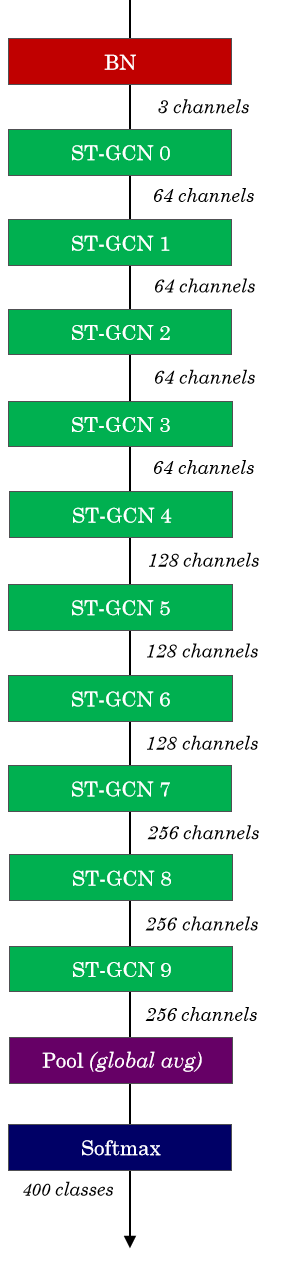
\includegraphics[width=2.5cm]{images/st_gcn_architecture}
    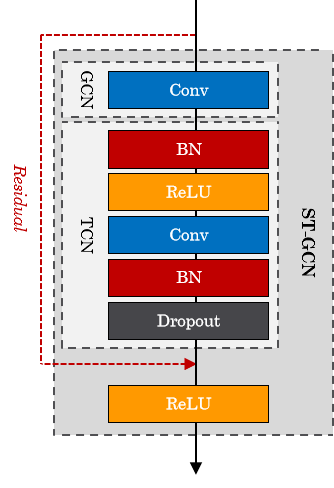
\includegraphics[width=3.0cm]{images/st_gcn_architeture_unit}
    \caption{Model architecture (left) and detail of one convolutional unit (right). ST-GCN layers apply normalization, convolution, activation, and dropout operations to the graphs and take into account the residual value of the previous layer to calculate the output activations. Adapted from \cite{st-gcn-2018}.}
    \label{fig:st-gcn-architecture}
\end{figure}

To estimate the skeletons of individuals in videos, in \cite{st-gcn-2018} the authors used a library called OpenPose. It is an open-source tool that uses deep learning algorithms to detect and estimate up to 130 human body points, as shown in figure \ref{fig:keypoints-openpose}, and which is presented in \cite{cao-realtime-2017, simon-hand-2017, wei-cpm-2016}.

\begin{figure}[ht]
    \centering
    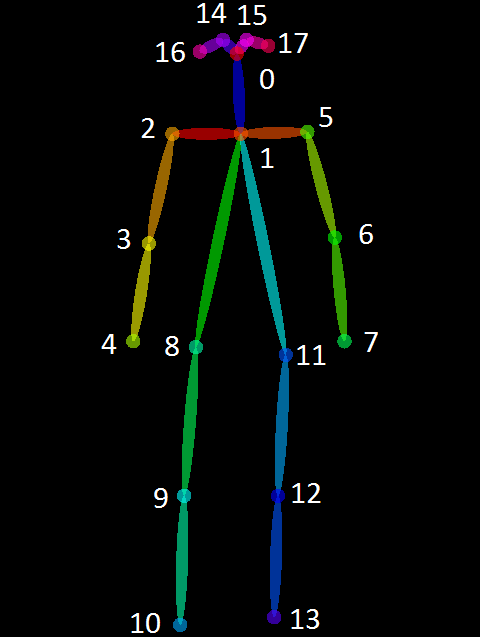
\includegraphics[width=2.5cm]{images/keypoints_pose_COCO_18}
    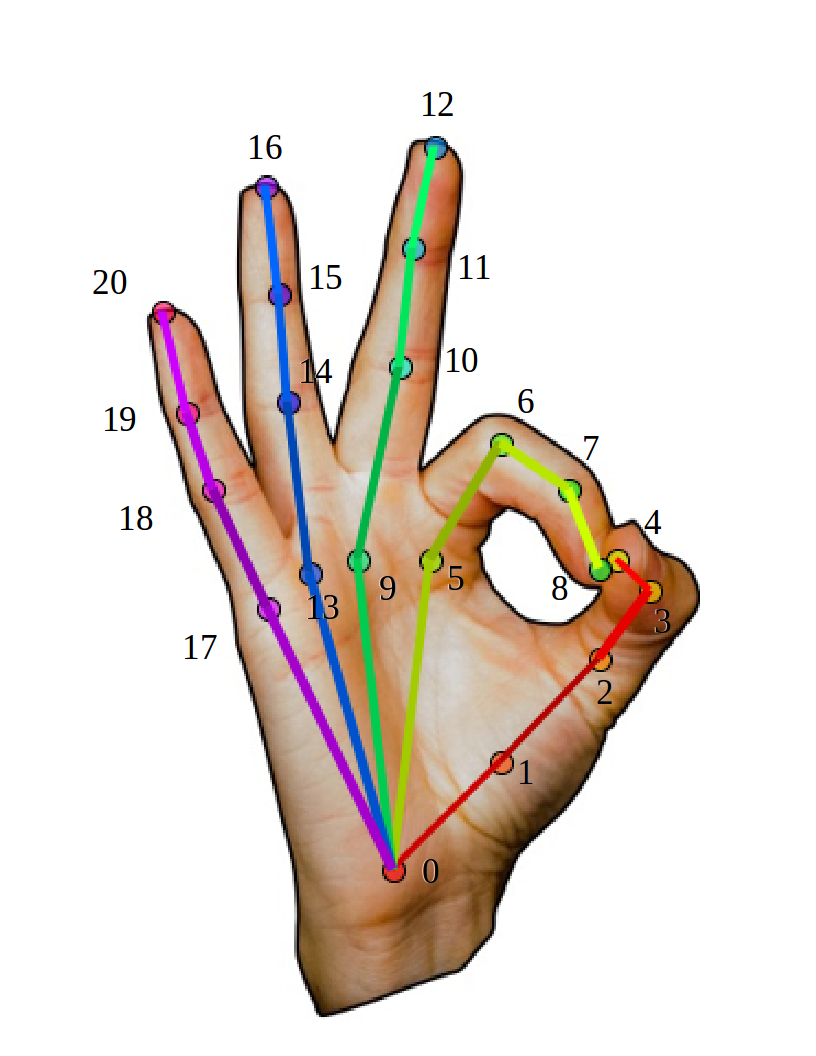
\includegraphics[width=2.5cm]{images/keypoints_hand}
    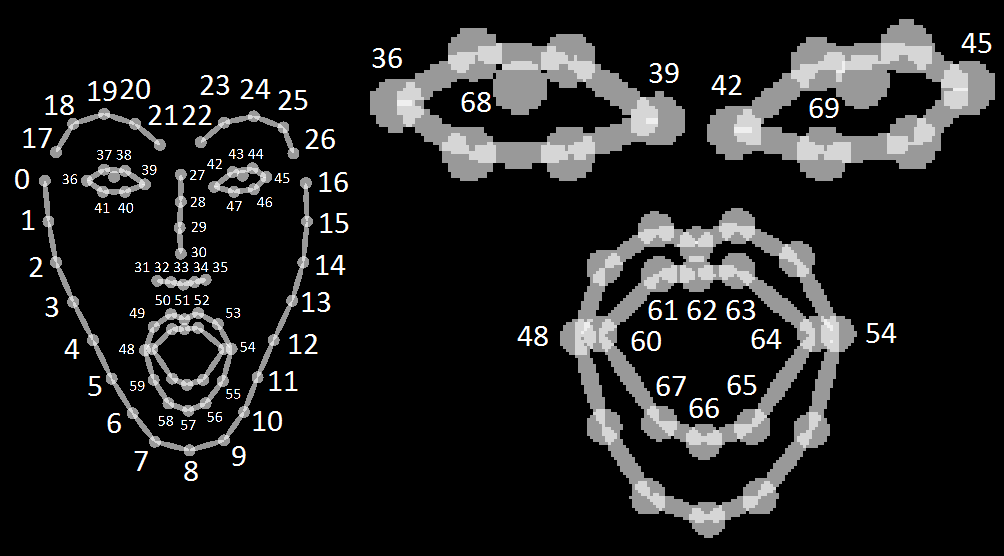
\includegraphics[width=3cm]{images/keypoints_face}
    \caption{Representation of the 130 points estimated by OpenPose, of which 18 correspond to the body (left); 21 correspond to each of the hands (center); and 70 points correspond to the face (right) \cite{openpose-output-2018}.}
    \label{fig:keypoints-openpose}
\end{figure}


%%%%%%%%%%%%%%%%%%%%%%%%%%%%%%%%%%%%%%%%%%%%%%%%%%%%%%%%%%%%%%%%%%%%%%%%%
\section{Experiments} 
\label{sec:experimentos}

This section presents the approach used to organize and conduct the experiments in this work. First, the ST-GCN was chosen as the model for its ability to focus primarily on human body movement, disregarding external environment interference, as best addressed in sections \ref{sec:introducao} and \ref{sec:trabalhos-relacionados}. These aspects are essential for techniques that propose to address the recognition of sign language, which also has the body dynamics as one of its central elements.

Next, the reference dataset has been established, as well as the preprocessing steps required to create a new ST-GCN compliant one, according to the problem addressed here. Finally, small adjustments were made to the model and the training to collect the results of this method was conducted.


%%%%%%%%%%%%%%%%%%%%%%%%%%%%%%%%%%%%%%%%%%%%%%%%%%%%%%%%%%%%%%%%%%%%%%%%%
\subsection{Dataset} 
\label{sec:dataset}

The American Sign Language Lexicon Video Dataset (ASLLVD) was chosen for this work. It consists of a large public dataset\footnote{
   Available at \url{http://csr.bu.edu/asl/asllvd/annotate/index.html}.
} containing video sequences of thousands of American Sign Language (ASL) signs, as well as their annotations, respective start and end frame markings, and class labels for each sample \cite{ athitsos-asllvd-2008, neidle-2012, vloger-2012}.

According to the authors, each sign is articulated by native individuals in ASL, and video sequences are collected using a four-camera system that simultaneously captures two frontal views, one side view and one enlarged view of the face of these individuals. Figure \ref{fig:asllvd-example} exemplifies capturing three of these views for the "MERRY-GO-ROUND" sign. 

\image
    {fig:asllvd-example}
    {images/asllvd_example}
    {Example of capture for the "MERRY-GO-ROUND" sign from three different perspectives, in the ASLLVD \cite[p. 2]{athitsos-asllvd-2008}.}
    
The number and type of signs included in ASLLVD are similar in scale and scope to the set of lexical entries in existing English-to-ASL dictionaries. There is at least one example of video per sign for almost all those contained in the Gallaudet Dictionary of American Sign Language \cite{athitsos-asllvd-2008, gallaudet-2005}.

By analyzing the dataset in detail it is possible to identify the existence of a total of 2,745 signs, represented in approximately 10 thousand samples. Each sign contains between 1 and 18 samples articulated by different individuals (where 4 is the average number of samples per sign).


%%%%%%%%%%%%%%%%%%%%%%%%%%%%%%%%%%%%%%%%%%%%%%%%%%%%%%%%%%%%%%%%%%%%%%%%%
\subsection{Creation of skeleton dataset for sign language} 
\label{sec:criacao-dataset}

In order to make the ASLLVD samples compatible with the input of the ST-GCN model, it was first necessary to apply a series of preprocessing steps, as shown in figure \ref{fig:preprocessamento}. These steps gave rise to a new dataset containing the estimate of the skeletons for all the signs contained therein.

The new skeleton dataset was named \textbf{ASLLVD-Skeleton}, and has been made publicly available\footnote{
   Available at \url{http://www.cin.ufpe.br/~cca5/asllvd-skeleton}
} in order to contribute to the development of future studies on the recognition of sign languages.

\image
    {fig:preprocessamento}
    {en/images/dataset_preprocessing}
    {Preprocessing steps for creating the ASLLVD-Skeleton dataset.}

The first step consists in \textbf{obtaining the videos} that make up the ASLLVD, in order to reconstitute the dataset and make feasible the later stages. A metadata file contained in it was used to guide this process. At this moment, only the videos captured by the frontal camera were considered, once they simultaneously contemplates movements of the trunk, hands and face of individuals.

The next step is to \textbf{segment the videos} to generate a video sample for each sign. Every file in the original dataset corresponds to a section where multiple signs were recorded per individual. Due to this, it is necessary to constitute a new set organized in such a way that each sign is arranged individually with its respective label. For this, we also considered the metadata file discussed above, which contains the labels and the start and end frame markings to perform the segmentation for each sign. The output of this step consists of small videos with average duration up to 5 seconds and looking similar to the one shown in figure \ref{fig:sign-original}.

\image
    [4cm]
    {fig:sign-original}
    {images/sign_original}
    {Representation of the "EXAGGERATE" sign, segmented from the sections recorded in ASLLVD.}

The third step consists of \textbf{estimating the skeletons} of the individuals present in the segmented videos. In other words, at this time the coordinates of the individuals' joints will be estimated for all frames, composing the skeletons that can be used later to generate the graphs of the ST-GCN. As in \cite {st-gcn-2018}, we used the OpenPose library in this process, and a total of 130 keypoints were estimated (according to figure \ref{fig:keypoints-openpose}). Figure \ref{fig:sign-pose} illustrates the reconstruction in a 2D image of the estimated coordinates for the "EXAGGERATE" sign.

\begin{figure}[ht]
    \centering
    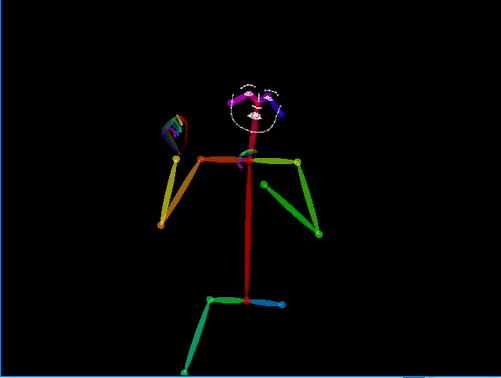
\includegraphics[width=3.5cm]{images/sign_pose}
    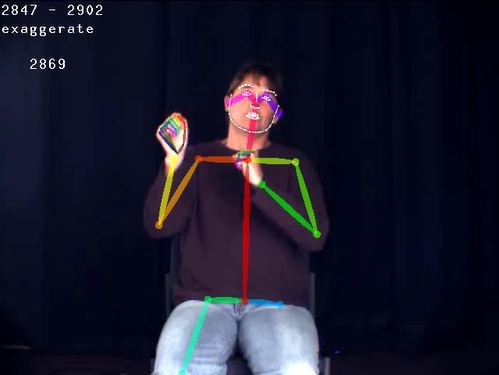
\includegraphics[width=3.5cm]{images/sign_pose_blended}
    \caption{Reconstruction of the skeleton from the coordinates estimated by OpenPose for the sign "EXAGGERATE" (left); and overlap of this skeleton in the original video (right).}
    \label{fig:sign-pose}
\end{figure}

Figure \ref{fig:openpose-coordinates} shows an example file obtained at the end of this step. In each frame, a section called "pose" with the coordinates of the X and Y axes estimated for  the body joints is contained, and a section "score" with the degree of confidence for each of these joints is also included.

\image
    [7.5cm]
    {fig:openpose-coordinates}
    {images/openpose_coordinates}
    {Example file containing the estimated coordinates for the skeletons in a sign. It includes a "pose" section with the X and Y coordinates of the estimated joints, and a "score" section with the respective degrees of confidence for each of them.}
    
% DONE: incluir passo de seleção de pontos
% explicar etapa
% falar do peso de rodar novamente o passo anterior ???
%   explicar pontos filtrados:
%   * 5 do corpo
%   * 11 de cada mão
% falar da saída (semelhante ao passo anterior, porém com menos pontos)
Then, the fourth step involves \textbf{filtering the keypoints} that will be used in this work. In the experiments presented below, only 27 of the 130 keypoints estimated in the previous step were considered, of which 5 refer to the shoulders and arms, and 11 refer to each of the individuals' hands, as ilustrated in figure \ref{fig:filtered-keypoints}. The output of this step consists of the same files obtained in the previous step, as shown in figure \ref{fig:openpose-coordinates}, but with a smaller number of coordinates per frame.

\begin{figure}[ht]
    \centering
    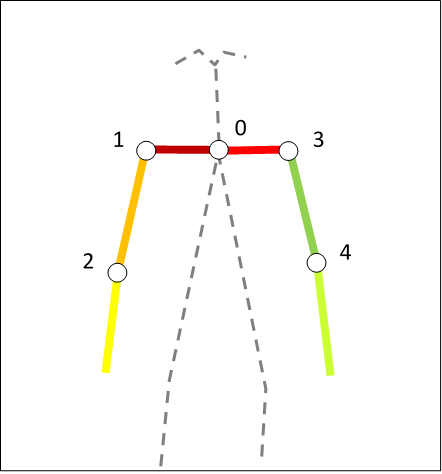
\includegraphics[width=3.5
    cm]{images/filtered_keypoints_body}
    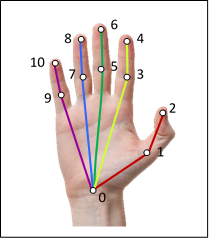
\includegraphics[width=3cm]{images/filtered_keypoints_hand}
    \caption{Representation of the 27 keypoints used in the experiments, of which 5 refer to the shoulders and arms (left) and 11 are refer to each of the hands (right).}
    \label{fig:filtered-keypoints}
\end{figure}


The fifth step concerns the \textbf{division of the dataset} processed so far into smaller subsets that will be used for training and testing the model. For this procedure, a cross-validation dataset tool called "\textit{train\_test\_split}", which is made available by the Scikit-Learn \cite{scikit-learn} library, was used. In this division, a proportion of 80\% of the samples were assigned for training (corresponding to 7,798 items) and 20\% for tests (corresponding to 1,950 items). This is a commonly adopted proportion and we understand that the number of samples in these groups is sufficient to validate the performance of most machine learning models.

Finally, the sixth step is to \textbf{normalize and serialize} the samples in order to make them compatible with the ST-GCN reading format. Normalization aims to make the length of all samples uniform by applying repetition of their frames sequentially to the complete filling of an established fixed number of frames. The number of fixed frames adopted here is 63 (which at a rate of 30 FPS, corresponds to a video with an approximate duration of 2 seconds). Serialization, in turn, consists of preloading the normalized samples from the subsets created above to translate them into physical Python \cite{python} files, which contain their in-memory representations. This is the format used by the ST-GCN, and it is adopted to optimize the process of data loading. For each of the subsets divided in the previous step two physical files are generated: one containing the samples and other containing the labels for those samples.

The output of the processing of each of the above steps is made available individually in ASLLVD-Skeleton, as above. The source code that performs the processing of these steps is also available along with the ST-GCN adaptations detailed in the following section.


%%%%%%%%%%%%%%%%%%%%%%%%%%%%%%%%%%%%%%%%%%%%%%%%%%%%%%%%%%%%%%%%%%%%%%%%%
\subsection{ST-GCN adaptation for the recognition of sign language} 
\label{sec:adaptacao-st-gcn}

Since the graph representation approach adopted by the ST-GCN is very flexible, it was not necessary in this work to make modifications in the architecture of the model. Instead, only punctual adaptations to get him to consider the new coordinates for the sign language domain were required.

Thus, a new graph layout was established for this problem, contemplating the 27 articulations adopted here and their relations. In addition, for custom layouts like this to be considered by the model, the ability to read these layouts from a configuration file has been implemented. Finally, small adjustments were made to the training matrices and the test data reader to accommodate the dynamic dimensions of the new coordinates.

The source code containing these adaptations has been made publicly available\footnote{
    Available at \url{http://www.cin.ufpe.br/~cca5/st-gcn-sl}
}. This code consists of a \textit{forked} repository created from the one originally developed by the authors in \cite{st-gcn-2018}.


%%%%%%%%%%%%%%%%%%%%%%%%%%%%%%%%%%%%%%%%%%%%%%%%%%%%%%%%%%%%%%%%%%%%%%%%%
\subsection{Preparation of experiments} 
\label{experimentos}

In this work, we adopted as reference the experiments presented in \cite{lim-2016}, which evaluate the performance in recognition of the ASLLVD dataset by the Block-Based Histogram of Optical Flow (BHOF) method (see section \ref{sec:trabalhos-relacionados}) and also by popular techniques such as Motion Energy Image (MEI) \cite{athitsos-asllvd-2008}, Motion History Image (MHI) \cite{babu-2004}, Principal Component Analysis (PCA) \cite{dreuw-2012} and Histogram of Optical Flow (HOF) \cite{laptev-2008}.

For this purpose, the authors used a subset containing 20 signs selected from the ASLLVD, as presented in table \ref{tab:asllvd-20}. To reproduce this configuration, the skeletons estimated for these signs were selected from the ASLLVD-Skeleton dataset created in section \ref{sec:criacao-dataset}. 
After this, it was identified that among the selected items there were divergent articulations for the signs AGAIN, BASEBALL, CAN, CHAT, CHEAP, CHEAT, CONFLICT, DEPRESS, DOCTOR and DRESS. In order to solve this, we chose to keep only that articulation that contained the largest number of samples for their respective signs.

Since the number of samples resulting from this process was small, totaling 131 items, it was necessary to apply a new division making 77\% of this subset to be separated for training and 33\% for tests. With this, a greater balance in the number of samples was obtained for an adequate evaluation of the model. Finally, as a new division of the samples was made, it was also necessary to normalize and serialize them to be compatible with the ST-GCN. In this process the same procedure as in section \ref{sec:criacao-dataset} was performed. The resulting subset was made publicly available\footnote{
    Available at \url{http://www.cin.ufpe.br/~cca5/asllvd-skeleton-20}
} and was named \textbf{ASLLVD-Skeleton-20}.

\begin{table}[ht]
\caption{Selected signs for the experiments in \cite{lim-2016}.}
\label{tab:asllvd-20}
\begin{tabular}{ll}
\hline
Dataset & Selected signs \\ \hline
ASLLVD & \begin{tabular}[c]{@{}l@{}}adopt, again, all, awkward, baseball, behavior, can, chat, \\ cheap, cheat, church, coat, conflict, court, deposit, depressed, \\ doctor, don’t want, dress, enough\end{tabular} \\ \hline
\end{tabular}
\end{table}

Still due to the characteristics of this small dataset, the size of the batch used in the training had to be reduced so that better results could be observed in the experiments. Thus, after a few failed attempts with larger batches, a batch size of 8 samples was considered.

In the same way as in the original implementation of the ST-GCN training algorithm in \cite {st-gcn-2018}, the experiments in this work used as optimizer the Stochastic Gradient Descent (SGD) with Nesterov Momentum, which in turn is able to improve stability and the convergence of the SGD, as described by \cite{stanford-2018, bengio-2013, sutskever-2013}.

% DONE: ajustar learning rate
For the learning rate, a strategy of initializing it with a higher value was applied so that the random weights were put in the direction of convergence within the first epochs. Then, this rate was gradually reduced in later epochs, allowing for more and more refined adjustments of training weights. Thus, in the experiment with the 20 selected signs, a total of 200 epochs were used, adopting an initial rate of 0.01, which was decreased to the values of 0.001, 0.0001 and 0.00001 after the end of the epochs 50, 100 and 150, respectively.

% TODO: revisar configurações do experimento completo / se será incluído
In addition to training with the subset of 20 signs above, an experiment with the complete ASLLVD dataset was also conducted in order to establish a reference value for it. To do this, only the setting related to the batch size had to be changed. Thus, the new batch size for this scenario with 2,745 signs was 24 and the learning rate had similar behavior to the experiment above.
% To do this, only the settings related to the batch size and the decay epochs of the learning rate had to be changed. Thus, the new batch size for this scenario with 2.745 signs was 24 and the learning rate had similar behavior to the experiment above.

The results obtained in both scenarios are presented in the following section, and the pre-trained models are available along with the adaptations made in the ST-GCN, according to section \ref{sec:adaptacao-st-gcn}.
% The results obtained are presented in the following section, and the pre-trained models are available along with the adaptations made in the ST-GCN, according to section \ref{sec:adaptacao-st-gcn}.


%%%%%%%%%%%%%%%%%%%%%%%%%%%%%%%%%%%%%%%%%%%%%%%%%%%%%%%%%%%%%%%%%%%%%%%%%
\section{Results} 
\label{sec:resultados}

The first experiment was performed using the approach presented in \cite{lim-2016}, which considers the selection of 20 specific signs of the ASLLVD, whose performance is represented in figure \ref{fig:training-asllvd-20}. The red line presents the accuracy of the model (\textit{top-1}), and its evolution over the course of training epochs. The gray line represents the \textit{top-5} accuracy, which corresponds to the accuracy based on the 5 most likely responses presented by the model. Finally, the blue dashed line represents the evolution of the learning rate used in the respective epochs, and its decay behavior.

\image
    [8.5cm]
    {fig:training-asllvd-20}
    {images/results_20}
    {Accuracy obtained by the presented approach in the recognition of the 20 signs selected from the ASLLVD. The red line represents the \textit{top-1} accuracy during the training periods; the gray line, the \textit{top-5} accuracy; and the blue dashed line illustrates the learning rate and its decay in the respective epochs.}

It can be observed from the image that the model was able to achieve an accuracy of 56.82\% from the epoch 80 in sign recognition. The \textit{top-5} accuracy, in turn, was able to reach 95.45\%. This performance was superior to the results presented by traditional techniques such as MEI, MHI and PCA, but was not able to overcome that obtained by the HOF and BHOF techniques \cite{lim-2016}. Table \ref{tab:results-comparison-20} presents the comparison of these results in detail.

\begin{table}[ht]
\centering
\caption{Accuracy in sign recognition using different approaches, as proposed in \cite{lim-2016}.}
\label{tab:results-comparison-20}
\begin{tabular}{lc}
\hline
                   & Accuracy (\%)  \\ \hline
MHI                & 10.00                     \\
MEI                & 25.00                     \\
PCA                & 45.00                     \\
\textbf{ST-GCN SL} & \textbf{56.82}            \\
HOF                & 70.00                     \\
BHOF               & 85.00                     \\ \hline
\end{tabular}
\end{table}

% TODO: revisar resultados do ASLLVD / se vai ser incluído
In order to establish a reference with the complete ASLLVD dataset, a second experiment was performed using its 2,745 signs. In this scenario, an accuracy (\textit{top-1}) of 20.85\% and a \textit{top-5} accuracy of approximately 40.15\% was observed. Of course, this is a much more challenging task than the one proposed in \cite{lim-2016} and these results clearly reflect this complexity.

% TODO: revisar justificativa (daqui para frente)
From the table, we can see that the approach presented in this paper, which is based on graphs of the coordinates of human articulations, has not yet been able to provide such remarkable results as that based on the description of the individual movement of the hands through histograms adopted by BHOF. Certainly, the application of consecutive steps for optical flow extraction, color map creation, block segmentation and generation of histograms from them were able to ensure that more enriched features about the hand movements were extracted favoring its sign recognition performance. This technique is derived from HOF and differs only by the approach of focusing on the hands of individuals while calculating the optical flow histogram.

Methods such as MEI and MHI, however, present more primitive approaches, which basically detect the movements and their intensity from the difference between the consecutive frames of actions. They are not able to differentiate individuals or to focus on specific parts of their body, causing movements of any nature to be considered equivalently. The PCA, in turn, adds the ability to reduce the dimensionality of the components based on the identification of those with greater variance and that, consequently, are more relevant for the detection of movement in the frames.

Although the results obtained with the presented approach did not reach an expressive performance, they are able to point the direction for the development of new studies. % For future work, it is understood that there is a need for a revision in the number of coordinates used, possibly leading to an assessment in the potential of each group to add significance to the domain of sign language recognition.
For future work, it is understood as relevant to adopt approaches that go in the direction of enriching the information about the movements of the coordinates, especially those of the hands and fingers, that play  fundamental roles in the articulation of the signs and which are more subtle to capture. Examples of this may be related to the creation of new partitioning strategies that emphasize the subtler movements of these parts to the detriment of those of the rest of the body; the definition of weights to be learned that favor these subtle movements; or the addition of depth data in the input coordinates, which would then contemplate the 3D plane.


%%%%%%%%%%%%%%%%%%%%%%%%%%%%%%%%%%%%%%%%%%%%%%%%%%%%%%%%%%%%%%%%%%%%%%%%%
% Bibliografia
\bibliographystyle{IEEEtran}
\bibliography{IEEEabrv,references.bib}

\end{document}